\documentclass[journal]{IEEEtran}
\usepackage{cite}
\usepackage{amsmath,amssymb,amsfonts}
\usepackage{graphicx}
\usepackage{textcomp}
\usepackage{xcolor}
\usepackage{booktabs}
\usepackage{url}
\usepackage{array}
\usepackage{siunitx}
% AUTO-GENERATED by Paper/generate_paper_assets.py from results/final/*.json - do not edit by hand
\newcommand{\nRaw}{572}
\newcommand{\nRawPatients}{500}
\newcommand{\nClinical}{493}
\newcommand{\nClinicalPos}{305}
\newcommand{\nMatched}{347}
\newcommand{\nMatchedPos}{237}
\newcommand{\nTrain}{277}
\newcommand{\nTest}{70}
\newcommand{\nProteinSamples}{352}
\newcommand{\nProteinRaw}{487}
\newcommand{\nProteinKept}{456}
\newcommand{\nPCAll}{129}
\newcommand{\nEvents}{9}
\newcommand{\nEventsTrain}{8}
\newcommand{\nEventsTest}{1}
\newcommand{\nEventsAll}{12}
\newcommand{\nFeatFull}{18}
\newcommand{\nFeatPreop}{13}
\newcommand{\nSites}{9}
\newcommand{\nSiteTotal}{384}
\newcommand{\nExternal}{109}
\newcommand{\bpLOC}{0.775}
\newcommand{\bpFL}{0.790}
\newcommand{\bpFR}{0.782}
\newcommand{\bpCEN}{0.789}
\newcommand{\bpBL}{0.723}
\newcommand{\bpFLminusLOC}{+0.015\ [\ensuremath{-}0.007, +0.037]}
\newcommand{\bpFRminusFL}{\ensuremath{-}0.008\ [\ensuremath{-}0.013, \ensuremath{-}0.003]}
\newcommand{\bpCENminusFL}{\ensuremath{-}0.001\ [\ensuremath{-}0.004, +0.002]}
\newcommand{\bpFLminusBL}{+0.067\ [+0.048, +0.086]}
\newcommand{\bpLcPartOne}{0.696}
\newcommand{\bpLcFrOne}{0.751}
\newcommand{\bpLcPartAll}{0.838}
\newcommand{\bpLcFrAll}{0.785}
\newcommand{\bpLooShapRho}{0.48\ [0.34, 0.62]}
\newcommand{\bpShapSizeRho}{0.51}
\newcommand{\bpMacroSites}{7.4}
\newcommand{\cvFull}{0.818}
\newcommand{\cvPreop}{0.642}
\newcommand{\cvProt}{0.574}
\newcommand{\cvFullProt}{0.659}
\newcommand{\cvSkFull}{0.824}
\newcommand{\cvRFFullProt}{0.782}
\newcommand{\cvRFFull}{0.803}
\newcommand{\cvProtDiff}{\ensuremath{-}0.159\ [\ensuremath{-}0.188, \ensuremath{-}0.130]}
\newcommand{\cvPreopDiff}{+0.176\ [+0.148, +0.203]}
\newcommand{\cvProtPreopDiff}{\ensuremath{-}0.047\ [\ensuremath{-}0.080, \ensuremath{-}0.013]}
\newcommand{\nFolds}{25}
\newcommand{\driftRedMin}{32.0}
\newcommand{\driftRedMax}{36.4}
\newcommand{\driftAvgIID}{0.206}
\newcommand{\driftAvgSkew}{0.770}
\newcommand{\driftMuZero}{0.599}
\newcommand{\driftMuOne}{0.268}
\newcommand{\sigmaTen}{5.68}
\newcommand{\sigmaFive}{10.55}
\newcommand{\sigmaTwo}{24.99}
\newcommand{\sigmaOne}{49.02}
\newcommand{\sigmaHalf}{97.01}
\newcommand{\auNoDP}{0.823}
\newcommand{\auAvgTen}{0.821}
\newcommand{\auProxTen}{0.823}
\newcommand{\auLossTen}{\ensuremath{-}0.002\ [\ensuremath{-}0.009, +0.005]}
\newcommand{\auAvgFive}{0.818}
\newcommand{\auProxFive}{0.821}
\newcommand{\auLossFive}{\ensuremath{-}0.005\ [\ensuremath{-}0.014, +0.003]}
\newcommand{\auAvgTwo}{0.800}
\newcommand{\auProxTwo}{0.812}
\newcommand{\auLossTwo}{\ensuremath{-}0.023\ [\ensuremath{-}0.038, \ensuremath{-}0.008]}
\newcommand{\auAvgOne}{0.761}
\newcommand{\auProxOne}{0.789}
\newcommand{\auLossOne}{\ensuremath{-}0.063\ [\ensuremath{-}0.087, \ensuremath{-}0.038]}
\newcommand{\auAvgHalf}{0.691}
\newcommand{\auProxHalf}{0.720}
\newcommand{\auLossHalf}{\ensuremath{-}0.132\ [\ensuremath{-}0.180, \ensuremath{-}0.085]}
\newcommand{\gridSup}{12}
\newcommand{\gridCells}{20}
\newcommand{\gridSupCtl}{3}
\newcommand{\gridNoDPmax}{0.0019}
\newcommand{\gridOneHalfMin}{0.028}
\newcommand{\gridOneHalfMax}{0.030}
\newcommand{\gridCtlOneHalfMax}{0.003}
\newcommand{\pflLocalThree}{0.754}
\newcommand{\pflProxThree}{0.811}
\newcommand{\pflPFLThree}{0.805}
\newcommand{\pflGainThree}{+0.051\ [+0.015, +0.086]}
\newcommand{\pflVsProxThree}{\ensuremath{-}0.006\ [\ensuremath{-}0.022, +0.011]}
\newcommand{\pflLocalFive}{0.796}
\newcommand{\pflProxFive}{0.817}
\newcommand{\pflPFLFive}{0.814}
\newcommand{\pflGainFive}{+0.018\ [\ensuremath{-}0.021, +0.057]}
\newcommand{\pflVsProxFive}{\ensuremath{-}0.003\ [\ensuremath{-}0.011, +0.005]}
\newcommand{\pflLocalTen}{0.785}
\newcommand{\pflProxTen}{0.841}
\newcommand{\pflPFLTen}{0.838}
\newcommand{\pflGainTen}{+0.053\ [+0.010, +0.096]}
\newcommand{\pflVsProxTen}{\ensuremath{-}0.003\ [\ensuremath{-}0.014, +0.007]}
\newcommand{\shRhoTenThree}{0.68}
\newcommand{\shRhoHalfThree}{0.25}
\newcommand{\shTSTenThree}{0.79}
\newcommand{\shTSHalfThree}{0.51}
\newcommand{\shRRHalfThree}{0.57}
\newcommand{\shLooThree}{0.68\ [0.42, 0.93]}
\newcommand{\shSizeThree}{0.55\ [0.31, 0.79]}
\newcommand{\shRThree}{5}
\newcommand{\shRhoTenFive}{0.66}
\newcommand{\shRhoHalfFive}{0.30}
\newcommand{\shTSTenFive}{0.65}
\newcommand{\shTSHalfFive}{0.41}
\newcommand{\shRRHalfFive}{0.74}
\newcommand{\shLooFive}{0.34\ [0.14, 0.54]}
\newcommand{\shSizeFive}{0.33\ [0.11, 0.55]}
\newcommand{\shRFive}{5}
\newcommand{\shRhoTenTen}{0.73}
\newcommand{\shRhoHalfTen}{0.36}
\newcommand{\shTSTenTen}{0.62}
\newcommand{\shTSHalfTen}{0.30}
\newcommand{\shRRHalfTen}{0.88}
\newcommand{\shLooTen}{0.44\ [0.30, 0.58]}
\newcommand{\shSizeTen}{0.46\ [0.35, 0.58]}
\newcommand{\shRTen}{2}
\newcommand{\miaNoDP}{0.511\ [0.489, 0.533]}
\newcommand{\miaOne}{0.510\ [0.484, 0.537]}
\newcommand{\miaHalf}{0.512\ [0.490, 0.534]}
\newcommand{\miaCtl}{0.659\ [0.640, 0.678]}
\newcommand{\miaGap}{+0.017\ [\ensuremath{-}0.007, +0.041]}
\newcommand{\shiftCovTwo}{0.765}
\newcommand{\shiftConTwo}{0.498}
\newcommand{\shiftBase}{0.826}
\newcommand{\abCen}{0.823}
\newcommand{\abAvg}{0.824}
\newcommand{\abProx}{0.826}
\newcommand{\abDPFive}{0.820}
\newcommand{\abDPOne}{0.787}
\newcommand{\abPreop}{0.659}
\newcommand{\abProt}{0.682}
\newcommand{\pNineN}{5{,}610}
\newcommand{\pNinePos}{2{,}146}
\newcommand{\pNineHosp}{19}
\newcommand{\pNineCountries}{8}
\newcommand{\pNinePrevLo}{12}
\newcommand{\pNinePrevHi}{60}
\newcommand{\pNinePrev}{38.3}
\newcommand{\pNineReps}{50}
\newcommand{\pRepNohBL}{0.827}
\newcommand{\pRepNohLOC}{0.818}
\newcommand{\pRepNohCEN}{0.827}
\newcommand{\pRepNohFL}{0.826}
\newcommand{\pRepNohFR}{0.827}
\newcommand{\pRepEttBL}{0.792}
\newcommand{\pRepEttLOC}{0.799}
\newcommand{\pRepEttCEN}{0.813}
\newcommand{\pRepEttFL}{0.803}
\newcommand{\pRepEttFR}{0.803}
\newcommand{\pSLOC}{0.829}
\newcommand{\pWLOC}{0.857}
\newcommand{\pSFL}{0.824}
\newcommand{\pWFL}{0.856}
\newcommand{\pSProx}{0.821}
\newcommand{\pWProx}{0.853}
\newcommand{\pSCEN}{0.825}
\newcommand{\pWCEN}{0.856}
\newcommand{\pSFR}{0.822}
\newcommand{\pWFR}{0.854}
\newcommand{\pSNoh}{0.834}
\newcommand{\pWNoh}{0.850}
\newcommand{\pSEtt}{0.795}
\newcommand{\pWEtt}{0.832}
\newcommand{\pDFLminusLOC}{\ensuremath{-}0.005\ [\ensuremath{-}0.015, +0.006]}
\newcommand{\pDFRminusFL}{\ensuremath{-}0.002\ [\ensuremath{-}0.002, \ensuremath{-}0.001]}
\newcommand{\pDCENminusFL}{+0.002\ [\ensuremath{-}0.001, +0.004]}
\newcommand{\pDFLminusNoh}{\ensuremath{-}0.010\ [\ensuremath{-}0.016, \ensuremath{-}0.005]}
\newcommand{\pDFLminusEtt}{+0.029\ [+0.023, +0.035]}
\newcommand{\pDProxminusFL}{\ensuremath{-}0.003\ [\ensuremath{-}0.005, \ensuremath{-}0.000]}
\newcommand{\pGainSig}{4}
\newcommand{\pLossSig}{4}
\newcommand{\pGainSizeRho}{\ensuremath{-}0.26}
\newcommand{\pLcFrOne}{0.769}
\newcommand{\pLcFrFive}{0.815}
\newcommand{\pLcFrLast}{0.830}
\newcommand{\pFrOE}{0.99}
\newcommand{\pFrSlope}{1.03}
\newcommand{\pDriftRed}{30.8}
\newcommand{\pDpLossHalf}{\ensuremath{-}0.005\ [\ensuremath{-}0.011, +0.001]}
\newcommand{\pDpLossOne}{\ensuremath{-}0.004\ [\ensuremath{-}0.008, +0.001]}
\newcommand{\pDpLossFive}{\ensuremath{-}0.002\ [\ensuremath{-}0.007, +0.003]}
\newcommand{\pProxHalfMax}{0.001}
\newcommand{\pSigmaHalf}{97}
\newcommand{\pPflSmall}{+0.039\ [+0.013, +0.065]}
\newcommand{\pPflAll}{+0.010\ [+0.005, +0.016]}
\newcommand{\pPflLarge}{+0.001\ [+0.000, +0.001]}
\newcommand{\pPflLargeLoc}{\ensuremath{-}0.005\ [\ensuremath{-}0.007, \ensuremath{-}0.004]}
\newcommand{\pNSmall}{4}
\newcommand{\pMiaNoDP}{0.500}
\newcommand{\pMiaCtl}{0.937}
\newcommand{\pLocoAvgNoh}{+0.001\ [\ensuremath{-}0.011, +0.012]}
\newcommand{\pLocoDpFive}{\ensuremath{-}0.005\ [\ensuremath{-}0.010, \ensuremath{-}0.000]}
\newcommand{\pLocoAvgCen}{\ensuremath{-}0.000\ [\ensuremath{-}0.001, +0.001]}
\newcommand{\pSlopeNoDP}{1.12\ [0.95, 1.30]}
\newcommand{\pSlopeDpFive}{0.81\ [0.70, 0.92]}
\newcommand{\pSlopeDpOne}{0.80\ [0.69, 0.91]}
\newcommand{\pSlopeNoh}{0.97\ [0.79, 1.14]}
\newcommand{\pRecalOeRaw}{0.263}
\newcommand{\pRecalOeInt}{0.071}
\newcommand{\pRecalOeDiff}{\ensuremath{-}0.193\ [\ensuremath{-}0.347, \ensuremath{-}0.038]}
\newcommand{\pRecalSlopeDpRaw}{0.81}
\newcommand{\pRecalSlopeDpLog}{0.99}
\newcommand{\pOeMin}{0.47}
\newcommand{\pOeMax}{1.30}
\newcommand{\pShRhoTen}{0.94}
\newcommand{\pShRhoHalf}{0.64}
\newcommand{\pShTSTen}{0.75}
\newcommand{\pShTSHalf}{0.40}
\newcommand{\pShRhoTwo}{0.91}
\newcommand{\pShRhoOne}{0.85}
\newcommand{\pShPhiMin}{0.029}
\newcommand{\pShPhiMax}{0.042}
\newcommand{\pShNineRhoFive}{0.90}
\newcommand{\pShNineRhoOne}{0.76}
\newcommand{\pShNineTSFive}{0.45}
\newcommand{\pShNineTSOne}{0.45}
\newcommand{\pShNineCoal}{1{,}777}
\newcommand{\pShLooRho}{0.66\ [0.56, 0.77]}
\newcommand{\pShSizeRho}{0.60}
\newcommand{\osaRhoTen}{0.90}
\newcommand{\osaRhoTwo}{0.89}
\newcommand{\osaRhoOne}{0.80}
\newcommand{\osaRhoHalf}{0.54}
\newcommand{\bmRhoTwo}{0.18}
\newcommand{\bmRhoTen}{0.47}
\newcommand{\bmRhoOne}{0.10}
\newcommand{\prRhoTen}{0.94}
\newcommand{\prRhoOne}{0.76}
\newcommand{\trueEpsOne}{33}
\newcommand{\trueEpsFive}{334}
\newcommand{\trueEpsTen}{988}
\newcommand{\osaVsBmTwo}{+0.71\ [+0.58, +0.84]}
\newcommand{\osaVsPrTwo}{\ensuremath{-}0.02\ [\ensuremath{-}0.06, +0.03]}
\newcommand{\osaVsPrOne}{+0.04\ [\ensuremath{-}0.05, +0.13]}
\newcommand{\osaNoDP}{0.96}
\newcommand{\osaSteps}{30}
\newcommand{\osaNineRhoFive}{0.95}
\newcommand{\osaNineRhoOne}{0.80}
\newcommand{\osaNineTSFive}{0.80}
\newcommand{\osaNineTSOne}{0.65}
\newcommand{\osaNineSize}{0.48}
\newcommand{\tOsaTwo}{0.39}
\newcommand{\tPrTwo}{0.52}
\newcommand{\tBmTwo}{\ensuremath{-}0.03}
\newcommand{\tOsaTen}{0.63}
\newcommand{\tPrTen}{0.72}
\newcommand{\tBmTen}{0.25}
\newcommand{\tOsaOne}{0.26}
\newcommand{\tPrOne}{0.44}
\newcommand{\tOsaNoDP}{0.91}
\newcommand{\mrRhoNoDP}{0.74}
\newcommand{\orRhoNoDP}{0.42}
\newcommand{\osaVsMrNoDP}{+0.22\ [+0.18, +0.27]}
\newcommand{\osaVsOrNoDP}{+0.54\ [+0.44, +0.65]}
\newcommand{\tMrRhoNoDP}{0.67}
\newcommand{\tOsaVsMrNoDP}{+0.24\ [+0.17, +0.31]}
\newcommand{\tHoOsaVsMrNoDP}{+0.29\ [+0.15, +0.42]}
\newcommand{\mrRhoTwo}{0.75}
\newcommand{\orRhoTwo}{0.51}
\newcommand{\osaVsMrTwo}{+0.14\ [+0.08, +0.19]}
\newcommand{\osaVsOrTwo}{+0.37\ [+0.26, +0.48]}
\newcommand{\tMrRhoTwo}{0.48}
\newcommand{\tOsaVsMrTwo}{\ensuremath{-}0.09\ [\ensuremath{-}0.27, +0.08]}
\newcommand{\tHoOsaVsMrTwo}{\ensuremath{-}0.23\ [\ensuremath{-}0.38, \ensuremath{-}0.09]}
\newcommand{\mrRhoOne}{0.65}
\newcommand{\orRhoOne}{0.50}
\newcommand{\osaVsMrOne}{+0.15\ [+0.03, +0.26]}
\newcommand{\osaVsOrOne}{+0.31\ [+0.18, +0.44]}
\newcommand{\tMrRhoOne}{0.39}
\newcommand{\tOsaVsMrOne}{\ensuremath{-}0.13\ [\ensuremath{-}0.32, +0.07]}
\newcommand{\tHoOsaVsMrOne}{\ensuremath{-}0.32\ [\ensuremath{-}0.51, \ensuremath{-}0.14]}
\newcommand{\mrRhoHalf}{0.37}
\newcommand{\orRhoHalf}{0.39}
\newcommand{\osaVsMrHalf}{+0.16\ [+0.04, +0.29]}
\newcommand{\osaVsOrHalf}{+0.14\ [+0.00, +0.28]}
\newcommand{\tMrRhoHalf}{0.26}
\newcommand{\tOsaVsMrHalf}{\ensuremath{-}0.07\ [\ensuremath{-}0.28, +0.15]}
\newcommand{\tHoOsaVsMrHalf}{\ensuremath{-}0.21\ [\ensuremath{-}0.46, +0.03]}
\newcommand{\mrRhoFive}{0.72}
\newcommand{\orRhoFive}{0.53}
\newcommand{\osaVsMrFive}{+0.18\ [+0.14, +0.22]}
\newcommand{\osaVsOrFive}{+0.37\ [+0.27, +0.47]}
\newcommand{\tMrRhoFive}{0.55}
\newcommand{\tOsaVsMrFive}{\ensuremath{-}0.03\ [\ensuremath{-}0.18, +0.12]}
\newcommand{\tHoOsaVsMrFive}{\ensuremath{-}0.12\ [\ensuremath{-}0.23, \ensuremath{-}0.00]}
\newcommand{\corrHosp}{es6}
\newcommand{\corrOsaTwo}{100\%}
\newcommand{\corrMrTwo}{70\%}
\newcommand{\corrOrTwo}{100\%}
\newcommand{\corrPrTwo}{100\%}
\newcommand{\corrBmTwo}{60\%}
\newcommand{\corrOsaOne}{95\%}
\newcommand{\corrMrOne}{80\%}
\newcommand{\corrOrOne}{100\%}
\newcommand{\corrPrOne}{100\%}
\newcommand{\corrBmOne}{45\%}
\newcommand{\corrTruth}{100\%}
\newcommand{\remOsa}{0.848}
\newcommand{\remMr}{0.849}
\newcommand{\remOr}{0.854}
\newcommand{\remTruth}{0.848}
\newcommand{\remRand}{0.853}
\newcommand{\remAll}{0.854}
\newcommand{\mlpOsaNoDP}{0.91}
\newcommand{\mlpParNoDP}{0.67}
\newcommand{\mlpMrNoDP}{0.78}
\newcommand{\mlpOsaVsMrNoDP}{+0.13\ [+0.07, +0.19]}
\newcommand{\mlpOsaTwo}{0.65}
\newcommand{\mlpParTwo}{0.65}
\newcommand{\mlpMrTwo}{0.82}
\newcommand{\mlpOsaVsMrTwo}{\ensuremath{-}0.17\ [\ensuremath{-}0.25, \ensuremath{-}0.09]}
\newcommand{\mlpOsaOne}{0.60}
\newcommand{\mlpParOne}{0.60}
\newcommand{\mlpMrOne}{0.78}
\newcommand{\mlpOsaVsMrOne}{\ensuremath{-}0.18\ [\ensuremath{-}0.29, \ensuremath{-}0.07]}
\newcommand{\mlpOsaFive}{0.68}
\newcommand{\mlpParFive}{0.52}
\newcommand{\mlpMrFive}{0.82}
\newcommand{\mlpOsaVsMrFive}{\ensuremath{-}0.14\ [\ensuremath{-}0.19, \ensuremath{-}0.09]}
\newcommand{\mlpOsaHalf}{0.42}
\newcommand{\mlpParHalf}{0.44}
\newcommand{\mlpMrHalf}{0.74}
\newcommand{\mlpOsaVsMrHalf}{\ensuremath{-}0.32\ [\ensuremath{-}0.46, \ensuremath{-}0.18]}
\newcommand{\mlpBmTwo}{0.16}
\newcommand{\mlpOsaVsBmTwo}{+0.47\ [\ensuremath{-}0.34, +1.28]}
\newcommand{\mlpTrueEpsTwo}{85}
\newcommand{\mlpBmOne}{0.05}
\newcommand{\mlpOsaVsBmOne}{+0.46\ [\ensuremath{-}0.42, +1.35]}
\newcommand{\mlpTrueEpsOne}{33}
\newcommand{\mlpBmSeeds}{5}
\newcommand{\blAvg}{0.816}
\newcommand{\blAvgLong}{0.818}
\newcommand{\blAdam}{0.818}
\newcommand{\blScaf}{0.816}
\newcommand{\blMLP}{0.821}
\newcommand{\blGB}{0.824}
\newcommand{\blRF}{0.820}
\newcommand{\blCMLP}{0.828}
\newcommand{\blCLR}{0.819}
\newcommand{\blDLong}{+0.002\ [+0.001, +0.003]}
\newcommand{\blDAdam}{+0.002\ [+0.000, +0.005]}
\newcommand{\blDMLP}{+0.005\ [+0.001, +0.009]}
\newcommand{\blDGB}{+0.009\ [+0.004, +0.014]}
\newcommand{\blDScaf}{\ensuremath{-}0.000\ [\ensuremath{-}0.001, +0.000]}
\newcommand{\blLMLP}{+0.005\ [\ensuremath{-}0.000, +0.010]}
\newcommand{\blLGB}{\ensuremath{-}0.003\ [\ensuremath{-}0.011, +0.004]}
\newcommand{\blScafDrift}{65}
\newcommand{\blProxDrift}{31}
\newcommand{\blDpScaf}{+0.000\ [\ensuremath{-}0.000, +0.000]}
\newcommand{\blDpAdam}{\ensuremath{-}0.004\ [\ensuremath{-}0.008, +0.000]}
\newcommand{\blDpProx}{\ensuremath{-}0.001\ [\ensuremath{-}0.004, +0.001]}
\newcommand{\btScafLow}{\ensuremath{-}0.004\ [\ensuremath{-}0.007, \ensuremath{-}0.001]}
\newcommand{\btAdamLow}{\ensuremath{-}0.016\ [\ensuremath{-}0.033, +0.001]}
\newcommand{\btMLPLow}{\ensuremath{-}0.013\ [\ensuremath{-}0.028, +0.001]}
\newcommand{\btAvgLow}{0.827}
\newcommand{\btScafMid}{+0.000\ [\ensuremath{-}0.002, +0.003]}
\newcommand{\btAdamMid}{\ensuremath{-}0.012\ [\ensuremath{-}0.025, +0.002]}
\newcommand{\btMLPMid}{\ensuremath{-}0.017\ [\ensuremath{-}0.030, \ensuremath{-}0.004]}
\newcommand{\btAvgMid}{0.822}
\newcommand{\btGB}{0.786}
\newcommand{\btCLR}{0.825}
\newcommand{\cvgFLminusLOC}{\ensuremath{-}0.005\ [\ensuremath{-}0.016, +0.006]}
\newcommand{\cvgFLminusNoh}{\ensuremath{-}0.008\ [\ensuremath{-}0.013, \ensuremath{-}0.003]}
\newcommand{\cvgFRminusFL}{\ensuremath{-}0.001\ [\ensuremath{-}0.001, \ensuremath{-}0.001]}
\newcommand{\cvgCENminusFL}{+0.001\ [\ensuremath{-}0.000, +0.003]}
\newcommand{\cvgFL}{0.826}
\newcommand{\cvgWFL}{0.858}
\newcommand{\cvgWNoh}{0.850}
\newcommand{\ssSigFull}{49.0}
\newcommand{\ssSigThree}{25.6}
\newcommand{\ssSigOne}{15.6}
\newcommand{\ssTThreeOne}{\ensuremath{-}0.009\ [\ensuremath{-}0.042, +0.025]}
\newcommand{\ssTThreeHalf}{\ensuremath{-}0.010\ [\ensuremath{-}0.070, +0.051]}
\newcommand{\ssTOneOne}{\ensuremath{-}0.009\ [\ensuremath{-}0.025, +0.008]}
\newcommand{\ssPThreeOne}{+0.001\ [\ensuremath{-}0.003, +0.004]}
\newcommand{\ssTFullOne}{0.761}
\newcommand{\ssTThreeOneAbs}{0.752}
\newcommand{\pxLSizeNoDP}{0.08}
\newcommand{\pxdLSizeNoDP}{+0.88\ [+0.79, +0.97]}
\newcommand{\pxLPosNoDP}{0.02}
\newcommand{\pxdLPosNoDP}{+0.94\ [+0.85, +1.03]}
\newcommand{\pxLStatNoDP}{\ensuremath{-}0.18}
\newcommand{\pxdLStatNoDP}{+1.14\ [+1.06, +1.21]}
\newcommand{\pxLOwnNoDP}{0.36}
\newcommand{\pxdLOwnNoDP}{+0.60\ [+0.44, +0.76]}
\newcommand{\pxLRefNoDP}{0.93}
\newcommand{\pxdLRefNoDP}{+0.03\ [+0.01, +0.05]}
\newcommand{\pxLLooNoDP}{0.85}
\newcommand{\pxdLLooNoDP}{+0.12\ [+0.08, +0.15]}
\newcommand{\pxLOsaNoDP}{0.96}
\newcommand{\pxLMrNoDP}{0.74}
\newcommand{\pxdLMrNoDP}{+0.22\ [+0.18, +0.27]}
\newcommand{\pxLOrNoDP}{0.42}
\newcommand{\pxdLOrNoDP}{+0.54\ [+0.44, +0.65]}
\newcommand{\pxLSizeFive}{0.08}
\newcommand{\pxdLSizeFive}{+0.82\ [+0.72, +0.92]}
\newcommand{\pxLPosFive}{0.02}
\newcommand{\pxdLPosFive}{+0.88\ [+0.78, +0.99]}
\newcommand{\pxLStatFive}{\ensuremath{-}0.18}
\newcommand{\pxdLStatFive}{+1.08\ [+1.00, +1.16]}
\newcommand{\pxLOwnFive}{0.26}
\newcommand{\pxdLOwnFive}{+0.64\ [+0.48, +0.80]}
\newcommand{\pxLRefFive}{0.88}
\newcommand{\pxdLRefFive}{+0.02\ [\ensuremath{-}0.01, +0.05]}
\newcommand{\pxLLooFive}{0.79}
\newcommand{\pxdLLooFive}{+0.12\ [+0.08, +0.15]}
\newcommand{\pxLOsaFive}{0.90}
\newcommand{\pxLMrFive}{0.72}
\newcommand{\pxdLMrFive}{+0.18\ [+0.14, +0.22]}
\newcommand{\pxLOrFive}{0.53}
\newcommand{\pxdLOrFive}{+0.37\ [+0.27, +0.47]}
\newcommand{\pxLSizeTwo}{0.08}
\newcommand{\pxdLSizeTwo}{+0.80\ [+0.70, +0.91]}
\newcommand{\pxLPosTwo}{0.02}
\newcommand{\pxdLPosTwo}{+0.87\ [+0.76, +0.97]}
\newcommand{\pxLStatTwo}{\ensuremath{-}0.18}
\newcommand{\pxdLStatTwo}{+1.06\ [+0.98, +1.15]}
\newcommand{\pxLOwnTwo}{0.25}
\newcommand{\pxdLOwnTwo}{+0.64\ [+0.49, +0.79]}
\newcommand{\pxLRefTwo}{0.85}
\newcommand{\pxdLRefTwo}{+0.04\ [\ensuremath{-}0.00, +0.08]}
\newcommand{\pxLLooTwo}{0.77}
\newcommand{\pxdLLooTwo}{+0.11\ [+0.08, +0.15]}
\newcommand{\pxLOsaTwo}{0.89}
\newcommand{\pxLMrTwo}{0.75}
\newcommand{\pxdLMrTwo}{+0.14\ [+0.08, +0.19]}
\newcommand{\pxLOrTwo}{0.51}
\newcommand{\pxdLOrTwo}{+0.37\ [+0.26, +0.48]}
\newcommand{\pxLSizeOne}{0.08}
\newcommand{\pxdLSizeOne}{+0.72\ [+0.61, +0.83]}
\newcommand{\pxLPosOne}{0.02}
\newcommand{\pxdLPosOne}{+0.78\ [+0.67, +0.90]}
\newcommand{\pxLStatOne}{\ensuremath{-}0.18}
\newcommand{\pxdLStatOne}{+0.98\ [+0.88, +1.08]}
\newcommand{\pxLOwnOne}{0.26}
\newcommand{\pxdLOwnOne}{+0.54\ [+0.42, +0.66]}
\newcommand{\pxLRefOne}{0.71}
\newcommand{\pxdLRefOne}{+0.10\ [+0.05, +0.14]}
\newcommand{\pxLLooOne}{0.74}
\newcommand{\pxdLLooOne}{+0.06\ [+0.01, +0.11]}
\newcommand{\pxLOsaOne}{0.80}
\newcommand{\pxLMrOne}{0.65}
\newcommand{\pxdLMrOne}{+0.15\ [+0.03, +0.26]}
\newcommand{\pxLOrOne}{0.50}
\newcommand{\pxdLOrOne}{+0.31\ [+0.18, +0.44]}
\newcommand{\pxSSizeNoDP}{0.74}
\newcommand{\pxdSSizeNoDP}{+0.21\ [+0.19, +0.24]}
\newcommand{\pxSPosNoDP}{0.50}
\newcommand{\pxdSPosNoDP}{+0.46\ [+0.43, +0.49]}
\newcommand{\pxSStatNoDP}{0.72}
\newcommand{\pxdSStatNoDP}{+0.23\ [+0.17, +0.29]}
\newcommand{\pxSOwnNoDP}{0.40}
\newcommand{\pxdSOwnNoDP}{+0.55\ [+0.45, +0.65]}
\newcommand{\pxSRefNoDP}{0.94}
\newcommand{\pxdSRefNoDP}{+0.01\ [\ensuremath{-}0.02, +0.03]}
\newcommand{\pxSLooNoDP}{0.59}
\newcommand{\pxdSLooNoDP}{+0.37\ [+0.28, +0.45]}
\newcommand{\pxSOsaNoDP}{0.95}
\newcommand{\pxSMrNoDP}{0.86}
\newcommand{\pxdSMrNoDP}{+0.10\ [+0.05, +0.14]}
\newcommand{\pxSOrNoDP}{0.79}
\newcommand{\pxdSOrNoDP}{+0.16\ [+0.12, +0.21]}
\newcommand{\pxSSizeFive}{0.74}
\newcommand{\pxdSSizeFive}{+0.11\ [+0.07, +0.16]}
\newcommand{\pxSPosFive}{0.50}
\newcommand{\pxdSPosFive}{+0.36\ [+0.31, +0.40]}
\newcommand{\pxSStatFive}{0.72}
\newcommand{\pxdSStatFive}{+0.13\ [+0.07, +0.19]}
\newcommand{\pxSOwnFive}{0.49}
\newcommand{\pxdSOwnFive}{+0.37\ [+0.23, +0.50]}
\newcommand{\pxSRefFive}{0.85}
\newcommand{\pxdSRefFive}{+0.00\ [\ensuremath{-}0.02, +0.02]}
\newcommand{\pxSLooFive}{0.36}
\newcommand{\pxdSLooFive}{+0.49\ [+0.40, +0.58]}
\newcommand{\pxSOsaFive}{0.85}
\newcommand{\pxSMrFive}{0.83}
\newcommand{\pxdSMrFive}{+0.03\ [\ensuremath{-}0.00, +0.06]}
\newcommand{\pxSOrFive}{0.81}
\newcommand{\pxdSOrFive}{+0.04\ [\ensuremath{-}0.00, +0.08]}
\newcommand{\pxSBmFive}{0.68}
\newcommand{\pxdSBmFive}{+0.17\ [+0.09, +0.25]}
\newcommand{\pxSSizeTwo}{0.74}
\newcommand{\pxdSSizeTwo}{+0.05\ [\ensuremath{-}0.01, +0.10]}
\newcommand{\pxSPosTwo}{0.50}
\newcommand{\pxdSPosTwo}{+0.29\ [+0.24, +0.35]}
\newcommand{\pxSStatTwo}{0.72}
\newcommand{\pxdSStatTwo}{+0.06\ [\ensuremath{-}0.01, +0.14]}
\newcommand{\pxSOwnTwo}{0.54}
\newcommand{\pxdSOwnTwo}{+0.24\ [+0.12, +0.36]}
\newcommand{\pxSRefTwo}{0.79}
\newcommand{\pxdSRefTwo}{\ensuremath{-}0.00\ [\ensuremath{-}0.06, +0.06]}
\newcommand{\pxSLooTwo}{0.34}
\newcommand{\pxdSLooTwo}{+0.44\ [+0.34, +0.54]}
\newcommand{\pxSOsaTwo}{0.79}
\newcommand{\pxSMrTwo}{0.78}
\newcommand{\pxdSMrTwo}{+0.00\ [\ensuremath{-}0.06, +0.06]}
\newcommand{\pxSOrTwo}{0.74}
\newcommand{\pxdSOrTwo}{+0.05\ [\ensuremath{-}0.03, +0.13]}
\newcommand{\pxSBmTwo}{0.45}
\newcommand{\pxdSBmTwo}{+0.34\ [+0.24, +0.44]}
\newcommand{\pxSSizeOne}{0.74}
\newcommand{\pxdSSizeOne}{\ensuremath{-}0.06\ [\ensuremath{-}0.15, +0.02]}
\newcommand{\pxSPosOne}{0.50}
\newcommand{\pxdSPosOne}{+0.18\ [+0.10, +0.27]}
\newcommand{\pxSStatOne}{0.72}
\newcommand{\pxdSStatOne}{\ensuremath{-}0.04\ [\ensuremath{-}0.15, +0.06]}
\newcommand{\pxSOwnOne}{0.56}
\newcommand{\pxdSOwnOne}{+0.12\ [\ensuremath{-}0.00, +0.24]}
\newcommand{\pxSRefOne}{0.72}
\newcommand{\pxdSRefOne}{\ensuremath{-}0.04\ [\ensuremath{-}0.10, +0.02]}
\newcommand{\pxSLooOne}{0.34}
\newcommand{\pxdSLooOne}{+0.34\ [+0.25, +0.44]}
\newcommand{\pxSOsaOne}{0.68}
\newcommand{\pxSMrOne}{0.74}
\newcommand{\pxdSMrOne}{\ensuremath{-}0.06\ [\ensuremath{-}0.15, +0.03]}
\newcommand{\pxSOrOne}{0.59}
\newcommand{\pxdSOrOne}{+0.09\ [\ensuremath{-}0.01, +0.19]}
\newcommand{\pxSBmOne}{0.29}
\newcommand{\pxdSBmOne}{+0.39\ [+0.25, +0.52]}
\newcommand{\pxCSizeNoDP}{0\%}
\newcommand{\pxCStatNoDP}{0\%}
\newcommand{\pxCOwnNoDP}{95\%}
\newcommand{\pxCRefNoDP}{100\%}
\newcommand{\pxCLooNoDP}{0\%}
\newcommand{\pxCOsaNoDP}{100\%}
\newcommand{\pxCSizeTwo}{0\%}
\newcommand{\pxCStatTwo}{0\%}
\newcommand{\pxCOwnTwo}{100\%}
\newcommand{\pxCRefTwo}{100\%}
\newcommand{\pxCLooTwo}{0\%}
\newcommand{\pxCOsaTwo}{100\%}
\newcommand{\pxCSizeOne}{0\%}
\newcommand{\pxCStatOne}{0\%}
\newcommand{\pxCOwnOne}{90\%}
\newcommand{\pxCRefOne}{100\%}
\newcommand{\pxCLooOne}{0\%}
\newcommand{\pxCOsaOne}{95\%}
\newcommand{\pxSmallMin}{16}
\newcommand{\pxSmallMax}{266}
\newcommand{\pxSmallHosp}{nl, it, es4, es5, de2, gb, es1, es8, es3, es2}
\newcommand{\accMcNineteenOne}{52}
\newcommand{\accMcTenOne}{34}
\newcommand{\accMcFiftyOne}{103}
\newcommand{\accFourOne}{2.9}
\newcommand{\accFourTwo}{6.1}
\newcommand{\hrSizeNoDP}{\ensuremath{-}0.38}
\newcommand{\hrdSizeNoDP}{+1.30\ [+1.12, +1.48]}
\newcommand{\hrStatNoDP}{\ensuremath{-}0.38}
\newcommand{\hrdStatNoDP}{+1.30\ [+1.12, +1.48]}
\newcommand{\hrOwnNoDP}{\ensuremath{-}0.18}
\newcommand{\hrdOwnNoDP}{+1.10\ [+0.84, +1.36]}
\newcommand{\hrRefNoDP}{0.76}
\newcommand{\hrdRefNoDP}{+0.16\ [\ensuremath{-}0.01, +0.33]}
\newcommand{\hrLooNoDP}{0.82}
\newcommand{\hrdLooNoDP}{+0.10\ [\ensuremath{-}0.00, +0.20]}
\newcommand{\hrOsaNoDP}{0.92}
\newcommand{\hrMrNoDP}{0.70}
\newcommand{\hrdMrNoDP}{+0.22\ [+0.05, +0.39]}
\newcommand{\hrOrNoDP}{0.23}
\newcommand{\hrdOrNoDP}{+0.69\ [+0.46, +0.92]}
\newcommand{\hrSizeFive}{\ensuremath{-}0.38}
\newcommand{\hrdSizeFive}{+0.89\ [+0.51, +1.27]}
\newcommand{\hrStatFive}{\ensuremath{-}0.38}
\newcommand{\hrdStatFive}{+0.89\ [+0.51, +1.27]}
\newcommand{\hrOwnFive}{\ensuremath{-}0.17}
\newcommand{\hrdOwnFive}{+0.68\ [+0.28, +1.08]}
\newcommand{\hrRefFive}{0.42}
\newcommand{\hrdRefFive}{+0.09\ [\ensuremath{-}0.05, +0.23]}
\newcommand{\hrLooFive}{0.69}
\newcommand{\hrdLooFive}{\ensuremath{-}0.18\ [\ensuremath{-}0.39, +0.03]}
\newcommand{\hrOsaFive}{0.51}
\newcommand{\hrMrFive}{0.64}
\newcommand{\hrdMrFive}{\ensuremath{-}0.13\ [\ensuremath{-}0.38, +0.12]}
\newcommand{\hrOrFive}{0.29}
\newcommand{\hrdOrFive}{+0.22\ [+0.01, +0.43]}
\newcommand{\hrBmFive}{\ensuremath{-}0.02}
\newcommand{\hrdBmFive}{+0.53\ [+0.17, +0.89]}
\newcommand{\hrPrFive}{0.34}
\newcommand{\hrdPrFive}{+0.17\ [\ensuremath{-}0.18, +0.52]}
\newcommand{\hrSizeTwo}{\ensuremath{-}0.38}
\newcommand{\hrdSizeTwo}{+0.53\ [+0.28, +0.78]}
\newcommand{\hrStatTwo}{\ensuremath{-}0.38}
\newcommand{\hrdStatTwo}{+0.53\ [+0.28, +0.78]}
\newcommand{\hrOwnTwo}{\ensuremath{-}0.31}
\newcommand{\hrdOwnTwo}{+0.46\ [+0.19, +0.73]}
\newcommand{\hrRefTwo}{\ensuremath{-}0.04}
\newcommand{\hrdRefTwo}{+0.19\ [+0.05, +0.33]}
\newcommand{\hrLooTwo}{0.42}
\newcommand{\hrdLooTwo}{\ensuremath{-}0.27\ [\ensuremath{-}0.59, +0.05]}
\newcommand{\hrOsaTwo}{0.15}
\newcommand{\hrMrTwo}{0.45}
\newcommand{\hrdMrTwo}{\ensuremath{-}0.30\ [\ensuremath{-}0.59, \ensuremath{-}0.01]}
\newcommand{\hrOrTwo}{0.18}
\newcommand{\hrdOrTwo}{\ensuremath{-}0.03\ [\ensuremath{-}0.34, +0.28]}
\newcommand{\hrBmTwo}{\ensuremath{-}0.18}
\newcommand{\hrdBmTwo}{+0.33\ [+0.05, +0.61]}
\newcommand{\hrPrTwo}{\ensuremath{-}0.09}
\newcommand{\hrdPrTwo}{+0.24\ [\ensuremath{-}0.04, +0.52]}
\newcommand{\hrSizeOne}{\ensuremath{-}0.38}
\newcommand{\hrdSizeOne}{+0.20\ [+0.02, +0.38]}
\newcommand{\hrStatOne}{\ensuremath{-}0.38}
\newcommand{\hrdStatOne}{+0.20\ [+0.02, +0.38]}
\newcommand{\hrOwnOne}{\ensuremath{-}0.30}
\newcommand{\hrdOwnOne}{+0.12\ [\ensuremath{-}0.16, +0.40]}
\newcommand{\hrRefOne}{\ensuremath{-}0.34}
\newcommand{\hrdRefOne}{+0.16\ [\ensuremath{-}0.01, +0.33]}
\newcommand{\hrLooOne}{0.18}
\newcommand{\hrdLooOne}{\ensuremath{-}0.36\ [\ensuremath{-}0.68, \ensuremath{-}0.04]}
\newcommand{\hrOsaOne}{\ensuremath{-}0.18}
\newcommand{\hrMrOne}{\ensuremath{-}0.35}
\newcommand{\hrdMrOne}{+0.17\ [\ensuremath{-}0.05, +0.39]}
\newcommand{\hrOrOne}{0.04}
\newcommand{\hrdOrOne}{\ensuremath{-}0.22\ [\ensuremath{-}0.59, +0.15]}
\newcommand{\hrBmOne}{\ensuremath{-}0.15}
\newcommand{\hrdBmOne}{\ensuremath{-}0.03\ [\ensuremath{-}0.32, +0.26]}
\newcommand{\hrPrOne}{\ensuremath{-}0.27}
\newcommand{\hrdPrOne}{+0.09\ [\ensuremath{-}0.12, +0.30]}
\newcommand{\hrCOsaTwo}{100\%}
\newcommand{\hrCRefTwo}{100\%}
\newcommand{\hrCSizeTwo}{0\%}
\newcommand{\hrCOsaOne}{80\%}
\newcommand{\hrCRefOne}{85\%}
\newcommand{\hrCSizeOne}{0\%}
\newcommand{\hrN}{920}
\newcommand{\hrFeat}{20}
\newcommand{\hrAuc}{0.85}
\newcommand{\hrCorrupt}{Budapest}
\newcommand{\hrPhiMin}{0.085}
\newcommand{\hrPhiMax}{0.101}
\newcommand{\hrTrueOne}{2.9}
\newcommand{\hrTrueTwo}{6.1}
\newcommand{\nuLarge}{114}
\newcommand{\nuSmall}{45}
\newcommand{\nuHeart}{43}
\newcommand{\nuMlp}{26}
\newcommand{\nsCrossTwo}{21}
\newcommand{\nsCrossOneMax}{38}
\newcommand{\nsCrossOneMin}{26}
\newcommand{\nsSpear}{0.57}
\newcommand{\nsLowerCount}{5}
\newcommand{\nsAFortyFiveNu}{45}
\newcommand{\nsAFortyFiveTwo}{+0.18\ [+0.08, +0.29]}
\newcommand{\nsAFortyFiveOne}{+0.12\ [\ensuremath{-}0.04, +0.27]}
\newcommand{\nsATwentyEightNu}{28}
\newcommand{\nsATwentyEightTwo}{+0.12\ [+0.00, +0.24]}
\newcommand{\nsATwentyEightOne}{+0.04\ [\ensuremath{-}0.07, +0.16]}
\newcommand{\nsASeventeenNu}{17}
\newcommand{\nsASeventeenTwo}{\ensuremath{-}0.09\ [\ensuremath{-}0.20, +0.03]}
\newcommand{\nsASeventeenOne}{\ensuremath{-}0.18\ [\ensuremath{-}0.32, \ensuremath{-}0.03]}
\newcommand{\nsASixtyEightNu}{68}
\newcommand{\nsASixtyEightTwo}{+0.08\ [+0.00, +0.16]}
\newcommand{\nsASixtyEightOne}{+0.14\ [+0.02, +0.26]}
\newcommand{\nsBTwentyOneNu}{57}
\newcommand{\nsBTwentyOneTwo}{+0.07\ [\ensuremath{-}0.03, +0.18]}
\newcommand{\nsBTwentyOneOne}{+0.13\ [+0.01, +0.24]}
\newcommand{\nsBFiftyNu}{40}
\newcommand{\nsBFiftyTwo}{+0.05\ [\ensuremath{-}0.02, +0.12]}
\newcommand{\nsBFiftyOne}{+0.01\ [\ensuremath{-}0.08, +0.10]}
\newcommand{\nsBHundredNu}{29}
\newcommand{\nsBHundredTwo}{+0.05\ [\ensuremath{-}0.02, +0.11]}
\newcommand{\nsBHundredOne}{\ensuremath{-}0.07\ [\ensuremath{-}0.15, +0.00]}

\usepackage{xr}
\externaldocument[S-]{jbhi_supp}

\begin{document}

\title{The Hidden Privacy Cost of Valuing Hospitals in Federated Learning: Accounting, a Decision Rule, and Evidence from Real Federations}

\author{Ponnaluri~Jeyanth,
        Pudota~Jaideep,
        and~M.~V.~P.~Chandra~Sekhara~Rao%
\thanks{P. Jeyanth and P. Jaideep are with the Department of Computer Science and Engineering (Data Science), R.V.R. \& J.C. College of Engineering, Guntur, India (e-mail: jeyanthponnaluri08@gmail.com; pudotajaideep@gmail.com).}%
\thanks{M. V. P. Chandra Sekhara Rao is Professor and Head of the Department of Computer Science and Engineering (Data Science), R.V.R. \& J.C. College of Engineering, Guntur, India (e-mail: manukondach@gmail.com).}%
\thanks{Code, data provenance and all results: \protect\url{https://github.com/JeyanthPonnaluri/Mini_Project_RVR}.}}

\markboth{Manuscript submitted to IEEE Journal of Biomedical and Health Informatics}%
{Jeyanth \MakeLowercase{\textit{et al.}}: The Hidden Privacy Cost of Valuing Hospitals in Federated Learning}

\maketitle

\begin{abstract}
Hospitals that train a model together need to know what each contributes. Under differential privacy (DP), Shapley values are usually computed by retraining coalitions of hospitals, and the privacy cost of the valuation itself is rarely counted. This empirical study measures that cost and asks which valuations remain useful once it is paid honestly. The accounting is a direct consequence of standard DP composition: a hospital whose patients enter $r$ private runs pays for all of them, so with ten hospitals a reported per-run $\varepsilon=1$ costs $\varepsilon\approx\trueEpsOne$ for exact Shapley values and $\approx\accMcTenOne$ with 100 sampled permutations, and holding the true budget needs $\sqrt r$ times the noise, which destroys the ranking. We therefore compare valuations that only post-process releases whose cost is already counted (reconstruction from the DP training run, the basis of GTG-Shapley; a single-model score; and OSA-Shapley, a simple baseline that averages one DP-trained model per hospital) with cheap proxies such as hospital size, on two real federations: 19 prostate-cancer hospitals (\pNineN{} men) and four heart-disease hospitals (\hrN{} patients). No method wins everywhere. OSA-Shapley is the most accurate without DP, but under DP it leads only in the most favourable setting we studied, a seven-parameter logistic model on the ten largest prostate-cancer hospitals (Spearman $\rho=\osaRhoTwo$ with the exact ranking at $\varepsilon=2$, against \mrRhoTwo{} for reconstruction and \pxLSizeTwo{} for size); it ties reconstruction for small hospitals and loses to it for a neural network and in the heart-disease federation. Size and summary statistics are unreliable and never detect a hospital with random labels. Patients per hospital relative to the square root of the number of parameters predicts which valuation to use in direction; in an internally pre-registered test the predicted threshold was wrong, and we revise it. All models studied are low-dimensional tabular models.
\end{abstract}

\begin{IEEEkeywords}
Federated learning, contribution valuation, Shapley value, differential privacy, privacy accounting, prostate cancer, coronary artery disease.
\end{IEEEkeywords}

\section{Introduction}
\IEEEPARstart{R}{isk} calculators that decide, for example, whether a man with a raised PSA needs a prostate biopsy need data from many hospitals, but patient records cannot be pooled across institutions and countries. Federated learning (FL) lets hospitals train one model while records stay local \cite{Rieke2020DigitalHealth, McMahan2017FedAvg}. On 19 real prostate-cancer cohorts, large hospitals gained little from joining and non-contributors obtained almost the same model as contributors \cite{Kazlouski2025HospitalParticipation}, so a lasting federation needs a fair way to credit each hospital, for instance to share costs or rewards.

The Shapley value is the standard answer: the only allocation that is efficient, symmetric and gives nothing to a hospital that never helps \cite{Shapley1953, Ghorbani2019DataShapley}. Hospitals also need differential privacy (DP), because shared updates can reveal patients \cite{Shokri2017MIA, Abadi2016DPSGD}. The two interact badly. Exact Shapley values need a model for every coalition, and studies of valuation under DP usually retrain each coalition with DP-SGD and report a per-run budget. Every hospital then contributes its patients to $2^{K-1}$ private runs, so its real privacy loss is far larger than reported, and holding it at the stated budget requires so much noise that the ranking is lost. Hospitals could instead share sizes or summary statistics; whether such proxies suffice is an empirical question. Reconstructing coalition models from one training run \cite{Song2019BlockchainFL, Liu2022GTG} and re-using one private release \cite{Zhou2025Data} point to a way out, but neither has been evaluated on real hospitals at an honestly accounted budget. This is primarily an empirical study: its propositions are short consequences of standard DP facts (composition, post-processing and the variance of a weighted average), and its contribution lies in applying them, at an honestly counted budget, to real federations. Our contributions are:
\begin{itemize}
    \item \textbf{The hidden cost, made explicit.} The arithmetic is elementary, but it is rarely applied to valuation. Proposition~2 gives the composed cost of any retraining-based valuation in which a hospital's patients enter $r$ private runs, and the $\sqrt r$-fold noise needed to keep it honest (Table~\ref{tab:accounting}). A per-run $\varepsilon=1$ costs about \trueEpsOne{} for exact Shapley values over ten hospitals, and \accMcNineteenOne{} for 19 hospitals even with 100 sampled permutations.
    \item \textbf{A decision rule, tested in advance.} On two real federations without simulated silos we compare every valuation that costs the budget once, and proxies that cost nothing. Accuracy depends mainly on training patients per hospital relative to the square root of the number of parameters, the signal-to-noise ratio of a DP release (Proposition~3). We wrote down where the switch-over should lie before testing it; four of six internally pre-registered hypotheses held, the threshold did not, and we revise the rule.
    \item \textbf{OSA-Shapley, a simple baseline.} Combining one-shot averaging \cite{Zhang2013AVGM} with exact enumeration, each hospital releases one DP-trained model and every coalition model is the size-weighted average of these releases, so exact valuation of all $2^K$ coalitions costs the budget once (Proposition~1). It is the most accurate valuation without DP in every setting and, for the ten largest prostate-cancer hospitals, also under DP ($\rho=\osaRhoTwo$ at $\varepsilon=2$). Its advantage under DP is confined to this favourable setting; we do not claim it as a general-purpose method.
    \item \textbf{Honest negative results.} Size, case counts and summary statistics do not identify contributions reliably and never detect bad data; with few patients per parameter OSA-Shapley loses to reconstruction (heart disease, a federated MLP).
\end{itemize}

\section{Related Work}
\label{sec:related}
Cross-silo FL trains clinical models across institutions \cite{Rieke2020DigitalHealth, Sheller2020MedicineFL, Li2021SurveyFLMedical}; hospitals differ in case mix, so local models drift \cite{Kairouz2021FLAdvances, Zhao2018NonIID}, which FedProx and SCAFFOLD address \cite{Li2020FedProx, Karimireddy2020Scaffold}. Real-silo benchmarks such as FLamby keep the natural hospital split \cite{Terrail2022FLamby}. DP bounds the influence of any record \cite{Dwork2006CalibratingNoise, Dwork2008DPSurvey}; DP-SGD clips per-record gradients and adds Gaussian noise \cite{Abadi2016DPSGD}, R\'enyi DP composes it tightly \cite{Mironov2017RDP}, and Poisson subsampling amplifies privacy \cite{Mironov2019SampledGaussian}.

The Shapley value \cite{Shapley1953} has been adapted to data valuation \cite{Ghorbani2019DataShapley, Jia2019KNNShapley} and to federated clients \cite{Song2019BlockchainFL, Wei2020DataValuation, Lyu2020FairnessFL}; leave-one-out gives near-zero value to redundant clients \cite{Ghorbani2019DataShapley}. Because it needs a model per coalition, federated valuation samples coalitions \cite{Maleki2013Bounding, Jia2020EfficientShapley} or reconstructs coalition models from one training run: the multi-round (MR) and one-round (OR) reconstructions of Song \emph{et al.}\ \cite{Song2019BlockchainFL} and their truncated Monte-Carlo approximation GTG-Shapley \cite{Liu2022GTG}. Zhou \emph{et al.}\ \cite{Zhou2025Data} show that independent DP noise makes data values unreliable and that re-using released private gradients avoids this at no extra privacy cost. Jaramillo Velez \emph{et al.}\ \cite{JaramilloVelez2026Beyond} evaluate contributions under secure aggregation, where the server sees only coalition aggregates, with marginal-difference scores that keep Shapley-like properties; their privacy notion is compatibility with secure aggregation rather than a DP bound on the valuation, which is the cost we count. Studies of valuation under DP usually retrain coalitions at a per-run budget; to our knowledge, retraining, reconstruction and other post-processing valuations have not been compared at the same true budget on real hospitals, nor against cheap proxies (Table~\ref{tab:lit_comparison}).

\begin{table}[t]
\caption{Position of this work. \emph{Cost counted}: the privacy cost of the valuation itself is accounted. $^{\ast}$Secure aggregation, no DP.}
\centering\scriptsize
\setlength{\tabcolsep}{3pt}
\begin{tabular}{lcccccc}
\toprule
Study & Real & DP & Valua- & Cost & vs recon- & vs cheap \\
 & hospitals & & tion & counted & struction & proxies \\
\midrule
McMahan \emph{et al.}\ \cite{McMahan2017FedAvg} & No & No & No & -- & -- & No \\
Abadi \emph{et al.}\ \cite{Abadi2016DPSGD} & No & Yes & No & -- & -- & No \\
Ghorbani \& Zou \cite{Ghorbani2019DataShapley} & No & No & Yes & -- & No & No \\
Song \emph{et al.}\ \cite{Song2019BlockchainFL} & No & No & Yes & -- & -- & No \\
Liu \emph{et al.}\ (GTG) \cite{Liu2022GTG} & No & No & Yes & -- & -- & No \\
Zhou \emph{et al.}\ \cite{Zhou2025Data} & No & Yes & Yes & Yes & No & No \\
Jaramillo Velez \emph{et al.}\ \cite{JaramilloVelez2026Beyond} & No & No$^{\ast}$ & Yes & -- & Yes & No \\
Kazlouski \emph{et al.}\ \cite{Kazlouski2025HospitalParticipation} & Yes & No & No & -- & -- & No \\
\textbf{This work} & \textbf{Yes} & \textbf{Yes} & \textbf{Yes} & \textbf{Yes} & \textbf{Yes} & \textbf{Yes} \\
\bottomrule
\end{tabular}
\label{tab:lit_comparison}
\end{table}

\section{Setting and Methods}
\label{sec:method}
\label{sec:system}
\subsection{Federation, Model and Privacy}
A federation has $K$ hospitals and a server. Hospital $k$ holds $n_k$ patients with features $x_i\in\mathbb R^d$ and outcome $y_i\in\{0,1\}$ and minimises the $L_2$-regularised ($\lambda=10^{-3}$) cross-entropy of a logistic model $p_i=\sigma(x_i^Tw+b)$; FedAvg averages local models with weights $n_k/n$ after $E$ local epochs. Privacy is patient-level (add/remove adjacency). Each per-patient gradient is clipped to norm $C$ and the released gradient is $\tilde g = (\sum_i \bar g_i + z)/n_k$, $z\sim\mathcal N(0,\sigma^2C^2I)$. Updates are full-batch, so no amplification is claimed, and every patient enters all $N=T\times E$ steps of its own hospital. The R\'enyi accountant gives
\begin{equation}
\epsilon = \min_{\alpha} \left\{ N \frac{\alpha}{2 \sigma^2} + \frac{\ln(1/\delta)}{\alpha - 1} \right\},
\end{equation}
which agrees with the closed form $\rho+2\sqrt{\rho\ln(1/\delta)}$, $\rho=N/(2\sigma^2)$, to 0.01\%. For $N=100$, $\delta=10^{-5}$: $\sigma=\sigmaTen, \sigmaFive, \sigmaTwo, \sigmaOne, \sigmaHalf$ for $\varepsilon=10, 5, 2, 1, 0.5$. Subsampled accounting is a sensitivity analysis (Supplementary Section~\ref{S-sec:methods_more}). Fig.~\ref{fig:architecture} summarises the system.

\begin{figure*}[!t]
    \centering
    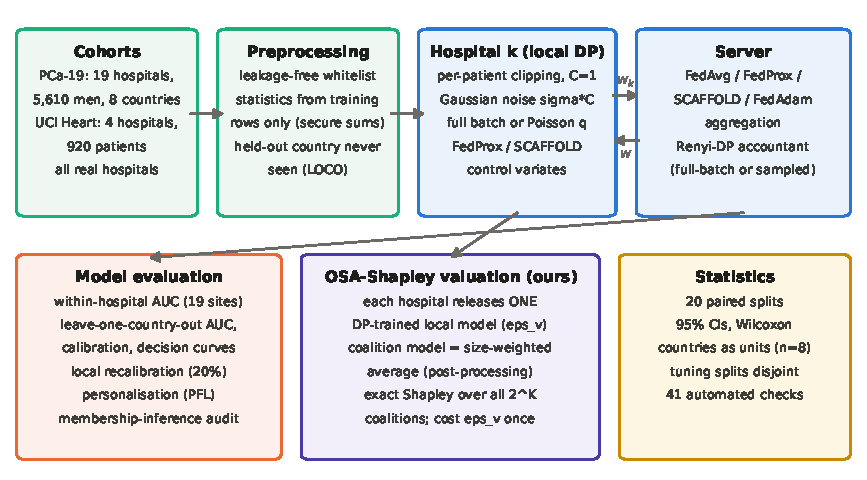
\includegraphics[width=0.85\textwidth]{figures/figure2_architecture.pdf}
    \caption{System architecture. Hospitals train locally with per-patient clipping and Gaussian noise and the server aggregates under a Rényi-DP accountant. The federated model is evaluated within hospitals and on held-out countries (Supplementary Material). Hospitals are valued with OSA-Shapley, which post-processes one DP-trained model per hospital, and compared with retraining and with reconstruction from the training run.}
    \label{fig:architecture}
\end{figure*}

\subsection{Shapley Valuation and Its Privacy Cost}
The Shapley value of hospital $k$ is
\begin{equation}
\phi_k = \sum_{S \subseteq \mathcal{N} \setminus \{k\}} \frac{|S|!(K - |S| - 1)!}{K!} \left[ v(S \cup \{k\}) - v(S) \right],
\end{equation}
where $v(S)$ is the AUC, on a reference set held by the server, of a model representing coalition $S$ ($v(\emptyset)=0.5$). For $K\le10$ we compute it \emph{exactly} by training all $2^K-1$ coalitions, so no Monte-Carlo error confounds the effect of DP. Under DP each coalition run draws independent noise, so this standard \emph{retraining} approach puts each hospital into $2^{K-1}$ private runs.

\emph{Proposition 2 (cost of retraining-based valuation).} Suppose a valuation trains $r_k$ DP models that use the patients of hospital $k$, each with $N$ full-batch Gaussian steps of multiplier $\sigma$. Then hospital $k$'s total RDP is that of a single run with multiplier $\sigma/\sqrt{r_k}$; keeping the total at the stated $(\varepsilon,\delta)$ requires multiplier $\sqrt{r_k}\,\sigma$ in every run. Exact Shapley values have $r_k=2^{K-1}$ (a factor of 22.6 for $K=10$); $M$ sampled permutations without caching have $r_k=M(K+1)/2$ on average.

\emph{Proof.} RDP of the Gaussian mechanism is $\alpha/(2\sigma^2)$ per step and composes additively, so $r_kN$ steps give $N\alpha/(2(\sigma/\sqrt{r_k})^2)$. In a random permutation hospital $k$ is equally likely at each of the $K$ positions and joins every later prefix, $(K+1)/2$ on average. $\square$

\begin{table}[t]
\caption{The privacy cost that retraining-based valuation actually spends (Proposition~2). $r$: number of DP training runs that contain a given hospital's patients (exact Shapley: $2^{K-1}$; permutation sampling without caching: on average $100(K+1)/2$). Each run is $N=100$ full-batch DP-GD steps calibrated to the per-run $\varepsilon$; the table gives the composed $\varepsilon$ per hospital ($\delta=10^{\ensuremath{-}5}$). Last column: factor by which every run's noise must grow to keep the stated budget ($\sqrt r$). Post-processing valuations spend the stated budget once.}
\centering\scriptsize
\setlength{\tabcolsep}{2.5pt}
\resizebox{\columnwidth}{!}{%
\begin{tabular}{lrccccr}
\toprule
 & & \multicolumn{4}{c}{True $\varepsilon$ for a per-run $\varepsilon$ of} & Noise \\
\cmidrule(lr){3-6}
Valuation & $r$ & 10 & 5 & 2 & 1 & factor \\
\midrule
Exact, $K=4$ & 8 & 36 & 16 & 6.1 & 2.9 & 2.8 \\
Exact, $K=10$ & 512 & 988 & 334 & 85 & 33 & 23 \\
Exact, $K=19$ & $\approx 10^{5}$ & $\approx 10^{5}$ & $\approx 10^{5}$ & 23{,}197 & 6{,}116 & 512 \\
Exact, $K=50$ & $\approx 10^{14}$ & $\approx 10^{14}$ & $\approx 10^{14}$ & $\approx 10^{13}$ & $\approx 10^{13}$ & $\approx 10^{7}$ \\
100 permutations, $K=10$ & 550 & 1{,}053 & 354 & 89 & 34 & 23 \\
100 permutations, $K=19$ & 1{,}000 & 1{,}820 & 597 & 141 & 52 & 32 \\
100 permutations, $K=50$ & 2{,}550 & 4{,}464 & 1{,}376 & 303 & 103 & 50 \\
OSA-Shapley, MR, OR (any $K$) & 1 & 10 & 5 & 2 & 1 & 1 \\
\bottomrule
\end{tabular}}
\label{tab:accounting}
\end{table}


Table~\ref{tab:accounting} evaluates Proposition~2. With 19 hospitals exact retraining is out of reach, and even 100 permutations cost $\varepsilon\approx\accMcNineteenOne$ per hospital; sampling reduces $r$ only for large $K$.

\subsection{OSA-Shapley}
\label{sec:osa}
We propose \emph{one-shot-averaging Shapley} (OSA-Shapley): (i) each hospital releases one model $\hat w_k$ trained locally by DP gradient descent at budget $\varepsilon_v$ (\osaSteps{} full-batch steps, $C=1$; the release averages the second half of the iterates); (ii) the server forms every coalition model as $w_S=\sum_{k\in S}(n_k/n_S)\hat w_k$, which for a convex model approximates the coalition's FedAvg solution \cite{Zhang2013AVGM}; (iii) $v(S)$ is the AUC of $w_S$ on the reference set, and exact Shapley values follow from all $2^K-1$ utilities. Only $K$ local trainings are needed; all 19 PCa-19 hospitals ($524{,}287$ coalitions) take about a minute on one CPU core. The number of local steps was chosen on four tuning splits disjoint from the evaluation splits. \emph{Approximation.} For i.i.d.\ data and smooth, strongly convex losses the one-shot average has mean-squared error $O(n^{-1} + (n/m)^{-2})$ for $n$ samples on $m$ sites \cite{Zhang2013AVGM}. Hospitals are not i.i.d., so we measure the approximation directly: without DP, OSA-Shapley reproduces the retraining Shapley ranking with $\rho=\osaNoDP$ for the ten largest and \pxSOsaNoDP{} for the ten smallest PCa-19 hospitals. \emph{Assumption.} As for retraining, the reference set is held by the server (for example a curated or consented validation set); the guarantees below protect the hospitals' training patients only, not the reference patients (Section~\ref{sec:discussion}).

\emph{Proposition 1 (privacy).} If each $\hat w_k$ is $(\varepsilon_v,\delta)$-DP with respect to the patients of hospital $k$, all utilities and Shapley values are jointly $(\varepsilon_v,\delta)$-DP with respect to every training patient, for any $K$. \emph{Proof.} Hospitals hold disjoint patients, so a patient affects one release, and everything else is a deterministic function of the releases and the reference set; DP is closed under post-processing \cite{Dwork2008DPSurvey}. $\square$

\emph{Proposition 3 (noise of coalition models).} If $\hat w_k=w_k+\xi_k$ with independent zero-mean $\xi_k$ of per-coordinate standard deviation at most $s_k=\eta\sigma C\sqrt N/n_k$ ($N$ steps of step size $\eta$), then
\begin{equation}
\mathrm{sd}(\hat w_S - w_S) = \frac{1}{n_S}\Big(\sum_{k\in S} n_k^2 s_k^2\Big)^{1/2} \le \frac{\eta\sigma C\sqrt{|S|\,N}}{n_S}.
\label{eq:prop3}
\end{equation}
\emph{Proof.} The variance of the weighted sum of independent terms is $\sum_{k\in S}(n_k/n_S)^2s_k^2$. $\square$

The coalition noise does not depend on $K$, whereas budget-matched retraining multiplies it by $2^{(K-1)/2}$; it is largest for a single small hospital and grows with the number of parameters (validation: observed 0.39--0.49 of the bound). Because all coalitions share the same releases, the noise is common to them and largely cancels in marginal contributions, the mechanism exploited by Zhou \emph{et al.}\ \cite{Zhou2025Data}.

\subsection{Competitors and Proxies at the Same Cost}
In DP-FedAvg each hospital releases a noisy model in every round, already covered by the accountant, so coalition models can be reconstructed at no extra cost. We implement the reconstructions of Song \emph{et al.}\ \cite{Song2019BlockchainFL} exactly: \emph{MR} sums, over rounds, exact Shapley values of $v_t(S)=\mathrm{AUC}(\sum_{k\in S}(n_k/n_S)\hat w_k^t)$, and is the idealised exact version of GTG-Shapley \cite{Liu2022GTG}; \emph{OR} rebuilds $w_S$ from the accumulated updates. Both use the DP-FedAvg run that trains the federated model. As proxies we use (i) hospital size, (ii) the number of cases, (iii) the similarity of summary statistics to the pooled ones, (iv) a self-reported AUC of the hospital's own model, (v) the AUC of its single DP release on the reference set and (vi) the leave-one-out value of the averaged releases; (v) and (vi) use OSA's releases and cost the same $\varepsilon$. Each valuation's ranking is compared with the exact non-private retraining Shapley ranking by Spearman's $\rho$, and we report how often a hospital given random labels is ranked last.

\subsection{Data and Protocol}
\label{sec:data}
\label{sec:silos}
\emph{PCa-19} is the patient-level collection of the base study, released under the MIT licence \cite{Kazlouski2025HospitalParticipation}: \pNineN{} men from \pNineHosp{} hospitals in eight countries (Table~\ref{S-tab:pca19_cohort}), \pNinePrev\% with clinically significant cancer (\pNinePrevLo--\pNinePrevHi\% per hospital). Features are age, $\log$ PSA, $\log$ prostate volume and PI-RADS 3/4/5 indicators, all available before biopsy; the logarithms keep the extreme PSA values of one hospital (median 277~ng/mL) from dominating. The base study's text states nine countries, but its released data contain eight; we use the released data unchanged, and for the reproduction of its protocol we use its exact Ettala and Noh variables. The \emph{UCI Heart Disease} collection \cite{Janosi1988HeartDisease, Detrano1989Heart} has \hrN{} patients referred for angiography at four hospitals (Cleveland 303, Budapest 294, Zurich/Basel 123, Long Beach 200); the target is coronary artery disease (prevalence 36--93\%), and preprocessing (Supplementary Section~\ref{S-sec:heart_prep}) gives \hrFeat{} features. OSA-Shapley keeps its PCa-19 settings, so this cohort is an out-of-sample test.

Every client is a real hospital as released; nothing is simulated or partitioned. Patients are split 80/20 within each hospital, stratified by outcome, with standardisation from training rows only. We value the ten largest (266--763 patients) and the ten smallest (\pxSmallMin--\pxSmallMax) PCa-19 hospitals, for which exact non-private references are computable (the Dutch hospital belongs to both groups), and all four heart-disease hospitals; the reference set is the pooled test patients. The ``useless hospital'' is a real hospital whose training labels are replaced by random labels (\corrHosp{}; \hrCorrupt{}). Settings: $T=20$, $E=5$, $\eta=0.5$, $\mu=0.5$, $C=1$, $\delta=10^{-5}$. Valuation results use 20 splits (seeds 20--39) not used for tuning; differences are paired by split and called significant only if the 95\% $t$-interval excludes zero.

\section{Results}
\label{sec:results}

\subsection{The Federation Being Valued}
\label{sec:federation}
Our re-implementation reproduces the base study's released code to within $1.2\times10^{-14}$, and its sustainability finding holds under our protocol: joining brings no significant average gain over local training (FL$-$LOC $=\pDFLminusLOC$) and a free-rider obtains almost the same model (FR$-$FL $=\pDFRminusFL$). DP changes the mean per-hospital AUC by only $\pDpLossHalf$ at $\varepsilon=0.5$ for this seven-parameter model. The model transports to held-out countries in discrimination but not in calibration (O/E \pOeMin--\pOeMax), which an intercept update on 20\% of a new country's patients largely fixes (Supplementary Section~\ref{S-sec:pca19_more}).

\subsection{Retraining Spends the Budget Hundreds of Times}
\label{sec:p19_retrain}
\label{sec:p19_osa}
Retraining every coalition of the ten largest hospitals at a per-run $\varepsilon$ looks accurate (Spearman $\rho=\pShRhoTen$ with the non-private ranking at $\varepsilon=10$, \pShRhoTwo{} at $\varepsilon=2$), but each hospital joins 512 runs, so a per-run $\varepsilon$ of 10, 5 or 1 is a total of about \trueEpsTen{}, \trueEpsFive{} and \trueEpsOne{} (Supplementary Table~\ref{S-tab:osa}). Held at the stated total (\emph{budget-matched}), $\rho$ falls to \bmRhoTen{} at $\varepsilon=10$ and \bmRhoOne{} at $\varepsilon=1$. OSA-Shapley spends the budget once and keeps $\rho=\osaNoDP$ without DP, \osaRhoTwo{} at $\varepsilon=2$ and \osaRhoOne{} at $\varepsilon=1$; at $\varepsilon=2$ it beats budget-matched retraining by $\osaVsBmTwo$ and matches per-run retraining ($\osaVsPrTwo$), which spends 28--42 times more privacy. All 19 hospitals can be valued exactly: the DP ranking agrees with the non-private one at $\rho=\osaNineRhoFive$ ($\varepsilon=5$) and \osaNineRhoOne{} ($\varepsilon=1$).

\subsection{Against Reconstruction and Cheap Proxies}
\label{sec:p19_post}
\label{sec:p19_proxies}
For the ten largest hospitals OSA-Shapley is more accurate than exact MR at every budget ($\rho$ \osaRhoTwo{} vs \mrRhoTwo{} at $\varepsilon=2$, difference \osaVsMrTwo; \osaRhoOne{} vs \mrRhoOne{} at $\varepsilon=1$) and beats OR by \osaVsOrTwo{} (Table~\ref{tab:proxies}; Supplementary Table~\ref{S-tab:osa_post}). The gap exists without DP ($\rho$ \osaNoDP{} vs \mrRhoNoDP), so it comes from the coalition proxy, not the noise.

Cheap proxies carry almost no information here: size, case counts and summary statistics reach $\rho$ \pxLSizeNoDP, \pxLPosNoDP{} and \pxLStatNoDP{} (OSA$-$size $=\pxdLSizeTwo$ at $\varepsilon=2$), because these hospitals differ in case mix and their value depends on what the others provide; a self-reported AUC is unverifiable and weak ($\rho=\pxLOwnTwo$). A score built on the released models is much better: the single-release AUC reaches $\rho=\pxLRefTwo$ at $\varepsilon=2$, and OSA-Shapley is comparable there ($\pxdLRefTwo$) and better at $\varepsilon=1$ ($\pxdLRefOne$), at no extra privacy cost and with values that are proper Shapley values. 

\begin{table*}[t]
\caption{Is OSA-Shapley worth its cost? Agreement (Spearman $\rho$) of cheap contribution proxies and of privacy-honest valuations with the exact non-private retraining Shapley ranking, on real PCa-19 hospitals (20 held-out splits). \emph{What is shared}: what each hospital must reveal. Proxies that use a model use the same DP releases as OSA-Shapley and therefore cost the same $\varepsilon$; size, counts and statistics are shared without DP. \emph{Useless}: share of splits in which a hospital whose training labels were replaced by random labels (es6) is ranked last at $\varepsilon=2$; a tie for last place does not count.}
\centering\scriptsize
\setlength{\tabcolsep}{4pt}
\begin{tabular}{llccccccc}
\toprule
 & & \multicolumn{4}{c}{Ten largest hospitals} & \multicolumn{3}{c}{Ten smallest hospitals} \\
\cmidrule(lr){3-6}\cmidrule(lr){7-9}
Contribution score & What is shared & no DP & $\varepsilon=2$ & $\varepsilon=1$ & Useless & no DP & $\varepsilon=2$ & $\varepsilon=1$ \\
\midrule
Hospital size $n_k$ & size (public) & 0.08 & 0.08 & 0.08 & 0\% & 0.74 & 0.74 & 0.74 \\
Number of csPCa cases & one count & 0.02 & 0.02 & 0.02 & 0\% & 0.50 & 0.50 & 0.50 \\
Similarity of summary statistics & feature means, prevalence & \ensuremath{-}0.18 & \ensuremath{-}0.18 & \ensuremath{-}0.18 & 0\% & 0.72 & 0.72 & 0.72 \\
Self-reported local AUC & one AUC (unverifiable) & 0.36 & 0.25 & 0.26 & 100\% & 0.40 & 0.54 & 0.56 \\
Single-model AUC on reference set & one DP model ($\varepsilon$) & 0.93 & 0.85 & 0.71 & 100\% & 0.94 & 0.79 & 0.72 \\
Leave-one-out of averaged models & one DP model ($\varepsilon$) & 0.85 & 0.77 & 0.74 & 0\% & 0.59 & 0.34 & 0.34 \\
OR reconstruction & DP-FedAvg run ($\varepsilon$) & 0.42 & 0.51 & 0.50 & 100\% & 0.79 & 0.74 & 0.59 \\
MR reconstruction (GTG bound) & DP-FedAvg run ($\varepsilon$) & 0.74 & 0.75 & 0.65 & 70\% & 0.86 & 0.78 & 0.74 \\
Retraining, budget-matched & $2^{K-1}$ runs ($\varepsilon$) & -- & 0.18 & 0.10 & 60\% & -- & 0.45 & 0.29 \\
\textbf{OSA-Shapley (ours)} & one DP model ($\varepsilon$) & \textbf{0.96} & \textbf{0.89} & \textbf{0.80} & 100\% & \textbf{0.95} & \textbf{0.79} & \textbf{0.68} \\
\bottomrule
\end{tabular}
\label{tab:proxies}
\end{table*}


\subsection{Small Hospitals}
To study small silos without simulating any, we value the ten smallest PCa-19 hospitals (\pxSmallMin--\pxSmallMax{} patients). Without DP OSA-Shapley is again the most accurate valuation ($\rho=\pxSOsaNoDP$; OSA$-$MR $=\pxdSMrNoDP$). Under DP its advantage disappears: at $\varepsilon=2$ OSA and MR agree with the ranking equally well (\pxSOsaTwo{} and \pxSMrTwo), and at $\varepsilon=1$ MR is slightly, not significantly, ahead (\pxdSMrOne); budget-matched retraining remains far worse ($\rho=\pxSBmTwo$). Here contribution follows volume, and size alone reaches $\rho=\pxSSizeNoDP$ (OSA$-$size $=\pxdSSizeTwo$ at $\varepsilon=2$). This is the regime Proposition~3 predicts: the release of a hospital with a few dozen patients carries noise of order $\sigma/n_k$, whereas reconstruction averages over the federation in every round.

\subsection{Useless Data and a Non-Convex Model}
\label{sec:p19_robust}
\label{sec:p19_small}
\label{sec:p19_mlp}
A hospital whose training labels were replaced by random labels (\corrHosp) is ranked last by the non-private reference in \corrTruth{} of splits; at $\varepsilon=2$ and 1 by OSA-Shapley in \corrOsaTwo{} and \corrOsaOne, by MR in \corrMrTwo{} and \corrMrOne, by budget-matched retraining in \corrBmTwo{} and \corrBmOne, and never by size or statistics. With a federated one-hidden-layer MLP (16 units; coalition prediction = size-weighted average of members' log-odds), OSA-Shapley is the most accurate valuation without DP ($\rho=\mlpOsaNoDP$ vs \mlpMrNoDP{} for MR) but loses under DP (\mlpOsaTwo{} vs \mlpMrTwo{} at $\varepsilon=2$; OSA$-$MR $=\mlpOsaVsMrTwo$): a network trained alone for 200 noisy steps accumulates the perturbation, whereas MR's short updates restart from the shared model every round (Supplementary Table~\ref{S-tab:osa_mlp}).

\subsection{A Second Real Federation: Heart Disease}
\label{sec:heart}
Without DP the heart-disease federation confirms the picture: OSA-Shapley recovers the exact ranking best ($\rho=\hrOsaNoDP$ vs \hrMrNoDP{} for MR; OSA$-$MR $=\hrdMrNoDP$; Table~\ref{tab:heart}). Under DP it does not. The hospitals have 98--242 training patients for 21 parameters and nearly equal contributions (Shapley values \hrPhiMin--\hrPhiMax{} AUC), so release noise dominates: at $\varepsilon=2$ MR is better (\hrMrTwo{} vs \hrOsaTwo; OSA$-$MR $=\hrdMrTwo$), and at $\varepsilon=1$ no valuation beats chance. Retraining does not help even at its modest composed cost here (a stated $\varepsilon=2$ costs \hrTrueTwo). Size is anti-correlated with contribution ($\rho=\hrSizeNoDP$), whereas OSA-Shapley and the single-release score still rank \hrCorrupt{} with random labels last in \hrCOsaTwo{} and \hrCRefTwo{} of splits at $\varepsilon=2$.

\begin{table}[t]
\caption{Second real federation: the four hospitals of the UCI Heart Disease collection (Cleveland (303), Budapest (294), Zurich/Basel (123), Long Beach VA (200) patients), coronary artery disease, 20 held-out splits. Spearman $\rho$ with the exact non-private retraining Shapley ranking; with four hospitals $\rho$ moves in steps of 0.2. Per-run retraining really costs $\varepsilon\approx16$, 6.1 and 2.9 at a stated 5, 2 and 1. \emph{Useless}: share of splits in which Budapest, given random training labels, is ranked last at $\varepsilon=2$.}
\centering\scriptsize
\setlength{\tabcolsep}{3pt}
\begin{tabular}{lccccc}
\toprule
Contribution score & no DP & $\varepsilon=5$ & $\varepsilon=2$ & $\varepsilon=1$ & Useless \\
\midrule
Hospital size $n_k$ & \ensuremath{-}0.38 & \ensuremath{-}0.38 & \ensuremath{-}0.38 & \ensuremath{-}0.38 & 0\% \\
Similarity of summary statistics & \ensuremath{-}0.38 & \ensuremath{-}0.38 & \ensuremath{-}0.38 & \ensuremath{-}0.38 & 0\% \\
Self-reported local AUC & \ensuremath{-}0.18 & \ensuremath{-}0.17 & \ensuremath{-}0.31 & \ensuremath{-}0.30 & 70\% \\
Single-model AUC on reference set & 0.76 & 0.42 & \ensuremath{-}0.04 & \ensuremath{-}0.34 & 100\% \\
Leave-one-out of averaged models & 0.82 & 0.69 & 0.42 & 0.18 & 85\% \\
OR reconstruction & 0.23 & 0.29 & 0.18 & 0.04 & -- \\
MR reconstruction (GTG bound) & 0.70 & 0.64 & 0.45 & \ensuremath{-}0.35 & -- \\
Retraining, per run & -- & 0.34 & \ensuremath{-}0.09 & \ensuremath{-}0.27 & -- \\
Retraining, budget-matched & -- & \ensuremath{-}0.02 & \ensuremath{-}0.18 & \ensuremath{-}0.15 & -- \\
\textbf{OSA-Shapley (ours)} & \textbf{0.92} & \textbf{0.51} & \textbf{0.15} & \textbf{\ensuremath{-}0.18} & 100\% \\
\bottomrule
\end{tabular}
\label{tab:heart}
\end{table}


\section{A Decision Rule, Tested in Advance}
\label{sec:rule}
By Proposition~3 the noise norm of a release over $p$ parameters scales as $\sqrt p/n_k$, so we index a setting by $\nu$, the median training patients per hospital divided by $\sqrt p$. OSA-Shapley won at $\nu=\nuLarge$ (ten largest PCa-19 hospitals) and not at $\nu\le\nuSmall$ (ten smallest \nuSmall, heart \nuHeart, MLP \nuMlp; Supplementary Table~\ref{S-tab:decision}), suggesting a switch-over between $\nu\approx50$ and 100.

\emph{Internally pre-registered test.} A threshold read off the results it explains is not evidence. Before running a new experiment we wrote down its design and six hypotheses and fixed them by a SHA-256 hash (Supplementary Section~\ref{S-sec:prereg}); the registration is internal, not public, and was written and run on the same day, so its timing cannot be verified independently and we treat the test as a prospectively specified internal check rather than a formal pre-registration. Within the ten largest hospitals we lowered $\nu$ by keeping 60--15\% of the training patients (arm A) or adding 21--100 uninformative features (arm B), each condition with its own exact reference (Fig.~\ref{fig:nu}).

The direction held but the threshold did not. As predicted, OSA-Shapley beat MR at $\nu\ge100$ (H1), its advantage shrank with $\nu$ (H3; Spearman \nsSpear), both arms agreed in sign (H5), and stronger privacy moved the switch-over up (H6). Contrary to H2 and H4, it kept a significant advantage down to $\nu\approx\nsAFortyFiveNu$ (OSA$-$MR $=\nsAFortyFiveTwo$ at $\varepsilon=2$) and fell behind only at $\nu\approx\nsASeventeenNu$; the mean difference changed sign at $\nu\approx\nsCrossTwo$ ($\varepsilon=2$) and \nsCrossOneMin--\nsCrossOneMax{} ($\varepsilon=1$). Four of six hypotheses held, and we revise the rule:

\begin{figure}[!t]
\centering
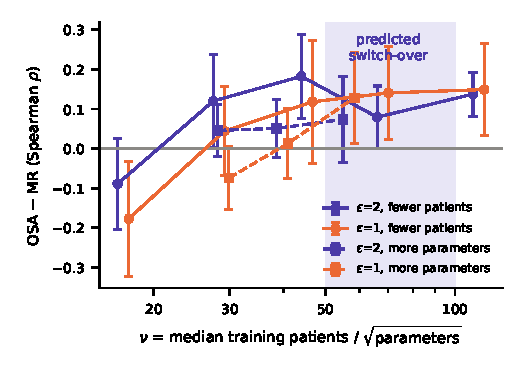
\includegraphics[width=\columnwidth]{figures/figure20_nu_sweep.pdf}
\caption{Internally pre-registered test: OSA$-$MR (paired difference in Spearman $\rho$ with the exact reference, 95\% CI, 20 splits) as $\nu$ is lowered within the ten largest PCa-19 hospitals, by removing patients (solid) or adding uninformative parameters (dashed). Shaded: the switch-over predicted before the test.}
\label{fig:nu}
\end{figure}

\begin{enumerate}
    \item \emph{Count the cost} of any valuation (Proposition~2); never retrain coalitions at a per-run budget.
    \item \emph{Without DP on the releases}, use OSA-Shapley, the most accurate valuation in all four settings.
    \item \emph{Under DP with a convex model}, OSA-Shapley is at least as accurate as MR down to $\nu\approx30$ ($\varepsilon=2$) and 40 ($\varepsilon=1$); below that use MR, which adds no cost when the federation trains with DP-FedAvg. \emph{With a non-convex model}, use MR.
    \item \emph{Check size before using it}: it matched contribution only where hospitals differed mainly in volume, and never detects bad data; a single released model's score does.
    \item \emph{When in doubt, compute both.} The heart-disease federation ($\nu=\nuHeart$) favoured MR although the sweep says OSA should be competitive; four hospitals make $\rho$ coarse and site-specific missing data leave single-hospital models poorly determined, both untested explanations. With small $\nu$ at $\varepsilon\le1$, equal shares plus screening for bad data is the honest fallback.
\end{enumerate}


\section{Discussion}
\label{sec:discussion}
The main lesson is about accounting. A hospital whose data enter $2^{K-1}$ coalition runs pays for all of them: on ten real hospitals a stated $\varepsilon=1$ becomes $\varepsilon\approx\trueEpsOne$, and when the budget is held honestly the ranking collapses. Payment or cost-sharing schemes built on such valuations either over-spend privacy or reward the wrong hospitals; valuation should post-process releases whose cost is already counted.

\emph{Is it practical?} OSA-Shapley asks each hospital for one DP-trained model, here seven numbers, the size of a single update in the DP-FedAvg run the federation performs anyway, and the coalition evaluations take about a minute for 19 hospitals. Sharing sizes or statistics is cheaper but unreliable: uninformative for the large prostate-cancer hospitals ($\rho\le\pxLSizeNoDP$), anti-correlated with contribution in the heart-disease federation ($\rho=\hrSizeNoDP$), and blind to useless data, because what a hospital adds depends on its case mix relative to the others. Within the privacy-honest class no method is best: single releases are as good as their noise, which grows with parameters and shrinks with patients, whereas reconstruction trades some bias for averaging over the whole federation in every round. We therefore avoid general statements about $\varepsilon$: the same budget barely changes the seven-parameter prostate calculator but degrades the heart-disease model and the MLP considerably.

\subsection{Threats to Validity}
\emph{Internal.} OSA-Shapley's local steps were tuned on four splits and evaluated on twenty disjoint ones. The exact non-private reference exists only for up to ten hospitals; for all 19 we report agreement with the non-private OSA ranking. PCa-19 was harmonised by the base study's authors from published supplementary files, and two hospitals have fewer than 50 patients.

\emph{External.} All evaluations are retrospective and use two federations and two clinical tasks; with four hospitals, $\rho$ moves in steps of 0.2, so the heart-disease estimates are coarse. One-shot averaging approximates the federated solution well for regularised logistic regression; for a federated MLP it is accurate without DP but loses under DP, and deeper networks are untested. All models are low-dimensional tabular models (logistic regression with 7--107 parameters and a 16-unit MLP); for imaging or other deep models $\nu$ is orders of magnitude smaller, our results suggest that OSA-Shapley would not be the right choice there, and the rule has not been tested in that regime. Shapley values depend on the reference population, and we have not tested a reference set from outside the federation.

\emph{Privacy.} The guarantee is per patient and treats hospital sizes and preprocessing statistics as public. OSA-Shapley's guarantee covers the valuation release; if the training run is also released, the two budgets compose. Like every Shapley method, it scores coalitions on a reference set held by the server, and the patients of that set are not protected: every utility $v(S)$ is a deterministic function of their records. Our experiments use the pooled test patients in this role, which is more than a real server would hold. In deployment the reference set should be public, consented for this use or itself privately released, or the utilities should be released with their own DP noise, whose cost then composes with $\varepsilon_v$; we have not evaluated these options.

\emph{Statistical.} Comparisons are paired over 20 splits of the same patients, so CIs describe variability across splits rather than across federations.

\subsection{Data, Code, Ethics and Conflicts}

Both data sets are public and de-identified and were used as released (PCa-19 \cite{Kazlouski2025HospitalParticipation}; UCI Heart Disease, doi:10.24432/C52P4X \cite{Janosi1988HeartDisease}); no ethics approval was required. The authors declare no conflicts of interest and received no external funding. Every number is regenerated from code, which passes 41 automated checks: \url{https://github.com/JeyanthPonnaluri/Mini_Project_RVR}.

\section{Conclusion}
\label{sec:conclusion}
Valuing hospitals by retraining coalitions under DP spends the privacy budget hundreds of times over and, at an honest budget, loses the ranking. Among valuations that pay once, none wins everywhere: OSA-Shapley is the most accurate without DP and, under DP, when hospitals hold many patients per parameter; reconstruction is better for a neural network and in the heart-disease federation; size and summary statistics are unreliable. Patients per hospital relative to $\sqrt{p}$ predicts the choice in direction, and an internally pre-registered test placed the switch-over near 30 at $\varepsilon=2$ and 40 at $\varepsilon=1$. OSA-Shapley should be read as a strong baseline for low-dimensional convex models, not as a general method. Explaining the heart-disease exception, testing the revised rule on a new federation under a public pre-registration, and OSA variants for neural networks are the next steps.

\bibliographystyle{IEEEtran}
\bibliography{references}

\end{document}
